

\spis{Jak przesłać bezpiecznie pierścionek zaręczynowy?}
{Piotr Chrząstowski-Wachtel}

\wtyt{\hspace*{-5.5cm}Jak przesłać bezpiecznie pierścionek zaręczynowy?}

\waut{Piotr CHRZĄSTOWSKI-WACHTEL*}
\aafil{Wydział Matematyki, Informatyki i~Mechaniki, Uniwersytet Warszawski}

Czemu przesyłać? Nie można dać osobiście? Otóż czasami nie można. Wyobraźmy
sobie sytuację, w~której więzień Artur (załóżmy, że niesłusznie oskarżony) chce
się oświadczyć swojej ukochanej Biance. Wykonał już pierścionek zaręczynowy, ale nie
może się z~nią spotkać. Na szczęście znalazł kuriera, który zobowiązał się
dostarczyć przesyłkę, ale nie jest to osoba godna zaufania. Nasz bohater  boi
się, że pierścionek może zostać skradziony, choć sam kurier
funkcjonuje na razie dobrze, skutecznie przekazując listy między zakochanymi. 

Artur wykonał również gustowną szkatułkę zamykaną na kłódki. Na szczęście ma ich
kilka i~na wszelki wypadek szkatułka została przygotowana tak, żeby można było zapiąć ją na
kilka kłódek. Mógłby więc włożyć pierścionek do szkatułki, zamknąć ją na kłódkę
i~wysłać kurierem, a następnie przesłać ukochanej kluczyk, którym będzie mogła otworzyć skrzynkę. Załóżmy jednak, że w kwestiach bezpieczeństwa Artur jest bardzo pryncypialny i z zasady nigdy nie powierza nikomu swoich kluczy. Czy przy takim ograniczeniu jest w stanie bezpiecznie wysłać Biance pierścionek?
% tylko jak przekazać kluczyk ukochanej?  Problem jest dokładnie ten sam, jak w~przypadku pierścionka: kluczyka nie może  przekazać przez kuriera, bo ten nadany kluczyk mógłby skopiować i~później użyć go do otwarcia szkatułki z~pierścionkiem. 

Artur ma następujący plan. Wysyła najpierw Biance instrukcję obsługi
-- w~instrukcji jest napisane, żeby Bianka kupiła kłódkę. Następnie wkłada
pierścionek do szkatułki i~zamyka ją na swoją kłódkę. Wysyła kurierem zamkniętą
szkatułkę bez kluczyka, a~Bianka, zgodnie z~instrukcją, zamyka szkatułkę na
drugą kłódkę i~odsyła bez swojego kluczyka całość do Artura. Teraz Artur
otrzymuje szkatułkę zamkniętą na dwie kłódki z~pierścionkiem w~środku. Otwiera
swoim kluczykiem swoją kłódkę i~odsyła szkatułkę Biance, a~ta może już
bezpiecznie otworzyć własną kłódkę. 
Kurier nigdy nie może otworzyć szkatułki, bo klucz nie wędruje
między stronami.\marg{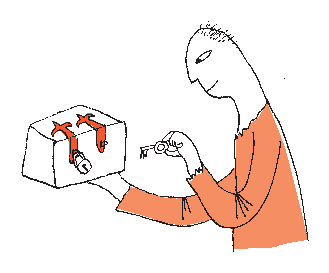
\includegraphics{art/202502_kol01}}

Wygląda na to, że ten algorytm mógłby być używany w~kryptografii. Jeśli chcemy
zakodować jakąś informację, możemy użyć klucza szyfrującego tak, aby potencjalny
podglądacz, powiedzmy właściciel pośredniczącego w~transmisji danych serwera,
nie mógł odczytać oryginału. Problem polega na tym, że zazwyczaj, aby
rozszyfrować zakodowany tekst, powinniśmy znać klucz. Przesłanie klucza może być
równie niebezpieczne, jak oryginalnej wiadomości~--
też może zostać
podglądnięty w~czasie transmisji danych. Z~kolei przekazanie klucza zawczasu
może być kłopotliwe albo wręcz niemożliwe. Ponadto, jeśli mamy do przekazania
duże dane, to w~niektórych protokołach szyfrujących może się okazać, że klucz
jest zbyt krótki i~zastosowanie go naraża naszą wiadomość na przykład na atak
statystyczny. 

\vspace*{\parskip}
\begin{dwieszpalty}\baselineskip12pt plus.1pt minus.2pt
\looseness-1{\spaceskip.33em minus.1em Zanim przejdziemy dalej, dwa słowa o~uwielbianej przez informatyków funkcji xor.
Jest to funkcja, która dla dwóch bitów daje jedynkę, jeśli są różne, a~zero,
jeśli są takie same. W~logice nazywana jest alternatywą wyłączającą (eXclusive~OR), a~w~podręcznikach oznaczana jest zwykle symbolem $\oplus$. Zauważmy, że jest
to funkcja przemienna: ${a \oplus b = b \oplus a}$ i~łączna: ${(a \oplus b)\oplus
c=a\oplus(b\oplus c)}$. Kolejność podania argumentów nie ma znaczenia, a~łączność
wynika z~zauważenia, że gdy ksorujemy więcej bitów, to wynik będzie równy jeden,
gdy liczba jedynek w~tym ciągu bitów jest nieparzysta, a~zero w~przeciwnym
razie. Grupowanie ich, w~ten czy inny sposób, nie zmieni wyniku. Czyli wynikiem
$(b_1\oplus...\oplus b_n)$ będzie 1 wtedy i~tylko wtedy, gdy będzie nieparzyście
wiele takich indeksów $k$, że $b_k=1$.}



Odnotujmy kilka podstawowych własności funkcji xor. Po pierwsze $a \oplus a = 0$. Po~drugie $0
\oplus a = a$. Po trzecie $a \oplus b \oplus a = b$. Ta ostatnia równość wynika
z~dwóch pierwszych, z~łączności i~z~przemienności. Po prostu $a  \oplus  b
\oplus  a = (b \oplus a) \oplus a = b \oplus (a \oplus a) = b \oplus 0 =
b$. 

To, co robimy na bitach, możemy też zrobić na ciągach bitów: dla dwóch jednakowej
długości ciągów  bitów możemy wykonać xor na każdej pozycji oddzielnie. Oznacza
to, że xor jest całkiem interesującą operacją arytmetyczną: jeśli będziemy
reprezentować liczby z~przedziału $[0,\dots,255]$ za pomocą jednego
bajtu~(czyli ciągu ośmiu bitów), to na
przykład $9 \oplus 5 =12$, gdyż 9 ma reprezentację dwójkową $00001001$, 5 ma
reprezentację $00000101$, a~12 ma reprezentację $00001100$ i~te jedynki
w~reprezentacji dwójkowej 12 są tam, gdzie reprezentacje 9 i~5 się różnią.
Oczywiście skoro $9 \oplus 5=12$, to $12 \oplus 5=9 $ i $12 \oplus 9=5$. 


Wykorzystując te własności, moglibyśmy zaszyfrować dowolny tekst, ksorując go
z~danym kluczem, a~odszyfrowanie go polegałoby na ponownym sksorowaniu z~tym
samym kluczem. Jeśli zatem
\end{dwieszpalty}

 odbiorca wiadomości, którą chcemy zaszyfrować, znałby
nasz
klucz, to tekst, który chcemy nadać, sksorowalibyśmy z~kluczem litera po
literze. Kiedy odbiorca drugi raz sksoruje zaszyfrowany tekst z~tym kluczem, to
odczyta oryginał. 


Powiedzmy, że umawiamy się, że naszym kluczem będą słowa inwokacji z~,,Pana
Tadeusza'' {\em Litwo, Ojczyzno moja! ty jesteś jak zdrowie}. Tekst ten ma 43~znaki. Zakodowany w~kodzie ASCII będzie miał 342~bity, które mogą być użyte do
ksorowania z~kolejnymi znakami szyfrowanego tekstu. Wynik, jaki dostaniemy,
raczej nie będzie przypominał oryginału.  Na przykład słowo {\em Delta\/},
mające w~kodzie ASCII wartości kolejnych liter równe [68][101][108][116][97]
sksorowane z~pierwszymi 5 znakami klucza, czyli słowem {\em Litwo\/} o~kodzie
ASCII [76][105][116][119][111], dałoby tekst,
\marg{Tak naprawdę nie istnieje tekst o~odczycie [8][12][24][3][14] w~kodzie
ASCII, gdyż kody odpowiadające ,,drukowalnym'' znakom znajdują się w~przedziale
od 32 do 126. Nic jednak nie stoi na przeszkodzie, by w~komunikacji wykorzystywać po
prostu ciągi liczb.}
który w~kodzie ASCII miałby reprezentację
[8][12][24][3][14], bo $68 \oplus 76=8$, $101\oplus
105=12$, $108\oplus 116 = 24,
116\oplus 119=3$, $97\oplus 111=14$. Rzecz jasna, ciąg
[8][12][24][3][14] sksorowany
z~ciągiem  [76][105][116][119][111], czyli słowem {\em Litwo\/}, da nam
z~powrotem ciąg [68][101][108][116][97], czyli słowo {\em Delta}. Są jednak wady
tego pomysłu.

Pierwsza -- przekazanie i~przechowywanie klucza: każda metoda jest wrażliwa na
ataki. Druga: może się okazać, że komunikat, który nadajemy, jest dłuższy niż
klucz. Wtedy oczywiście można po tylu pierwszych znakach, ile jest w~kluczu
(czyli 43 w~naszym przykładzie), ponownie zacząć od początku używać klucza, ale
jest w~tym pewien~problem. Okazuje się, że jeśli nasz zaszyfrowany tekst jest bardzo długi,
to w~tym momencie niektóre litery klucza zaczynają istotnie częściej być używane
do kodowania, a~inne rzadziej. Na przykład w~naszym kluczu są aż 4 litery {\em
o\/} i~nie ma żadnej litery {\em u}. Jeśli tekst, który chcemy zakodować, jest napisany
w~języku polskim, dla którego częstości występowania liter są nam znane, to
najczęściej występującą w~naszym języku literę \textit{a}~będziemy częściej kodowali za
pomocą \textit{o} niż jakąkolwiek inną literę zakodowaną jakimkolwiek innym znakiem.
Badając zaszyfrowany tekst, moglibyśmy znaleźć najczęściej występującą
zaszyfrowaną literę i~przyjąć, że jest to szyfr litery \textit{a}. W~ten sposób moglibyśmy odtworzyć najczęściej
występującą literę klucza i~tak po nitce do kłębka złamać cały klucz. 
Dlatego~dobrze byłoby, gdyby klucz miał długość równą długości zaszyfrowanego tekstu,
a~najlepiej, żeby dodatkowo był jakimś zupełnie losowym ciągiem znaków,
niemającym odpowiednika w~języku naturalnym. 

Możemy teraz przesyłać zaszyfrowane wiadomości, podobnie jak
Artur przesyłał pierścionek swojej ukochanej. Wystarczy bowiem kolejno: 

\begin{itemize}
 % \setlength{\itemsep}{2pt}  % Adjust the space between items
  \setlength{\parskip}{0pt}
\item wygenerować  losowy ciąg znaków o~długości równej długości tekstu, \item
sksorować go z~tekstem, który chcemy zaszyfrować, \item wysłać odbiorcy tekst
zakodowany kluczem, którego on nie zna, \item poprosić go o~wygenerowanie
swojego klucza, którego z~kolei my nie musimy znać, \item poprosić o~powtórne
zakodowanie zaszyfrowanego tekstu swoim losowo wygenerowanym kluczem
i~przesłanie nam podwójnie zakodowanego tekstu, \item otrzymany podwójnie
zakodowany tekst sksorować z~naszym kluczem, zdejmując jedno zakodowanie, ale
pozostawiając tekst zakodowany kluczem odbiorcy, \item przesłać odbiorcy wynik,
\item poprosić go o~sksorowanie ze swoim kluczem. \vadjust{\goodbreak} \end{itemize} Druga kłódka
zdjęta! Nadany  tekst został odczytany. Nikt po drodze nie widział ani
oryginalnego tekstu, ani klucza. Oba klucze możemy wyrzucić. No po prostu super! \marg{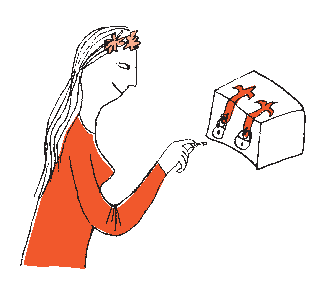
\includegraphics{art/202502_kol02}}

Niestety możemy wyrzucić do kosza też cały pomysł takiego szyfrowania. Zawiera
on bowiem pewien trudno usuwalny błąd. Nie tak łatwo go dostrzec na pierwszy
rzut oka. Problem w~tym, że oprócz zaszyfrowania wiadomości żądamy tego, aby
nikt, kto będzie podglądał transfer zaszyfrowanych tekstów, nie był w~stanie
odtworzyć  oryginału. Sprawdźmy, co by było, gdyby potencjalny podglądacz
przechwycił trzy zaszyfrowane teksty: pierwszy zaszyfrowany kluczem $a$ przez
Artura, drugi doszyfrowany kluczem $b$ przez Biankę i~trzeci odszyfrowany
kluczem $a$ przez Artura. Wtedy te trzy przesyłane teksty to kolejno $t
\oplus a$, $t\oplus a \oplus b$ oraz $t \oplus a \oplus b \oplus a = t \oplus b$. 

Sksorowanie tych trzech zaszyfrowanych wiadomości to ${(t \oplus a) \oplus (t
\oplus a \oplus b)}\allowbreak \oplus (t \oplus b)$, co z~uwagi na łączność i~przemienność
funkcji xor daje nam ${(t\oplus t) \oplus (a\oplus a) \oplus (b \oplus b) \oplus
t = 0\oplus 0 \oplus 0 \oplus t = t}$. Bez żadnego wysiłku z~tych trzech
tekstów odtworzymy zaszyfrowaną wiadomość $t$.

Zauważmy, 
\marg{Klasycznym rozwiązaniem naszego problemu w~kryptografii jest
\textit{protokół Diffiego--Hellmana} pozwalający ustalić stronom komunikacji
\textit{wspólny} klucz szyfrowania w~bezpieczny sposób.}
jak ważne w~kryptografii jest wyspecyfikowanie celu -- tu jest nim
niemożliwość lub wystarczająca trudność odtworzenia zaszyfrowanego tekstu przez
podglądacza bez znajomości kluczy szyfrujących. Tej istotnej własności niestety
naszej metodzie brakuje.  

A~najciekawsze jest to, że algorytm Artura z~fizycznymi kłódkami działa i~jest
nie do złamania, nawet jeśli kurier przez jakiś czas ma dostęp do zamkniętych
szkatułek.  \vskip-10pt

%\vskip2cm\mar
{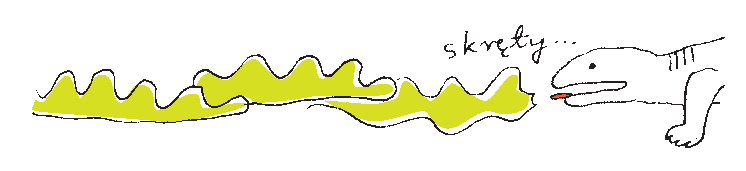
\includegraphics{art/202502_kol03}}
 \vskip-10pt
\input 02-miskiewicz
